% !TeX root = ../main.tex

\chapter{算法实现}

亏格测试数据采用 Blender 软件生成,通过 Cube 模型的布尔修改器得到,并导出为 obj 格式。实现代码均位于 \url{https://github.com/libreliu/GeoProcessing}。

计算最短同调圈的算法采用 Python 语言编写,使用 OpenMesh 处理网格,并采用 PyVista 进行网格可视化;计算柄圈的代码还额外用到了 TetGen \cite{Si2015} 及其封装 meshpy 库进行剖分,同时利用 ParaView 进行四面体网格可视化。

图 \ref{fig:genus2him} 展示了计算最短同调圈算法对 Genus2 模型的输出。

\begin{figure}[h]
    \centering
    \begin{subfigure}{.2\textwidth}
        \centering
        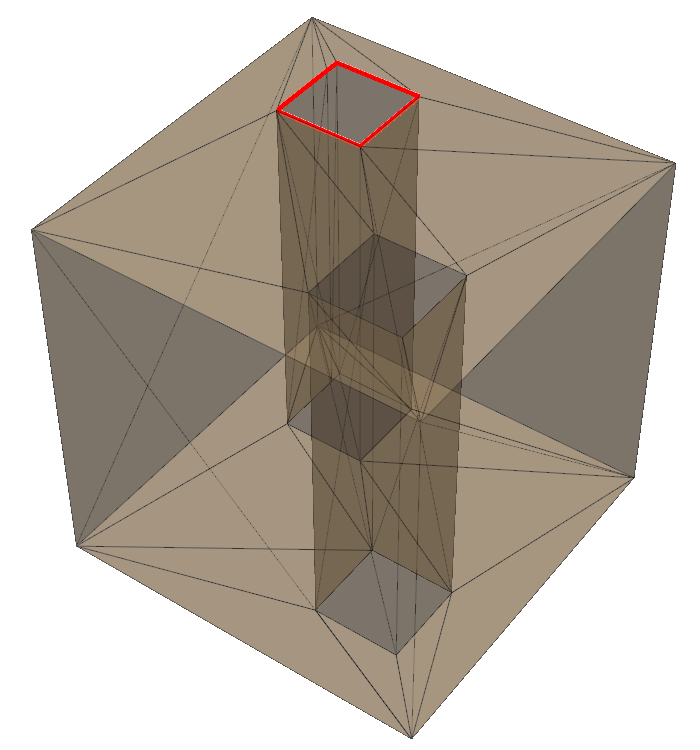
\includegraphics[width=\textwidth]{Genus2_0_optim_new.png}
        % \caption{提取经纬线前}
    \end{subfigure}
    \begin{subfigure}{.2\textwidth}
        \centering
        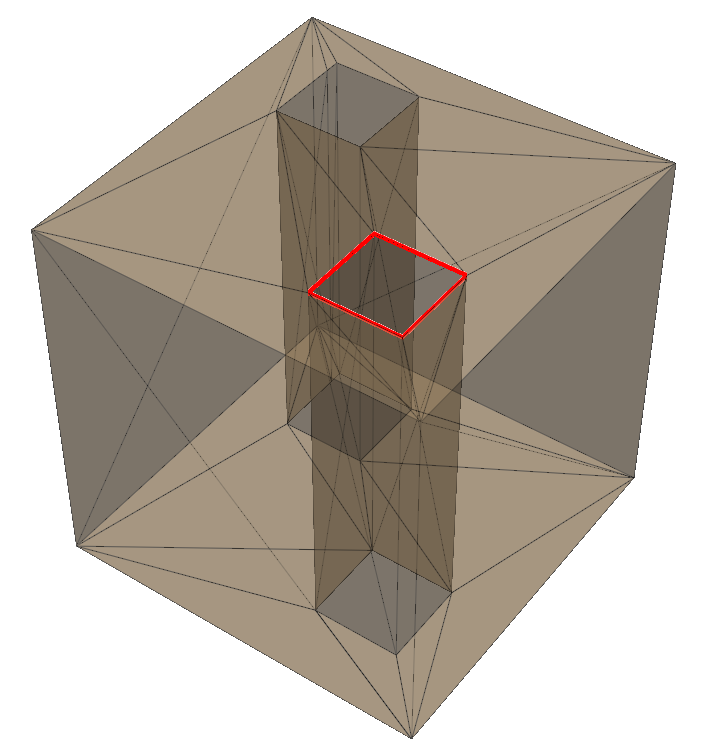
\includegraphics[width=\textwidth]{Genus2_1_optim_new.png}
        % \caption{提取经纬线后}
    \end{subfigure}
    \begin{subfigure}{.2\textwidth}
        \centering
        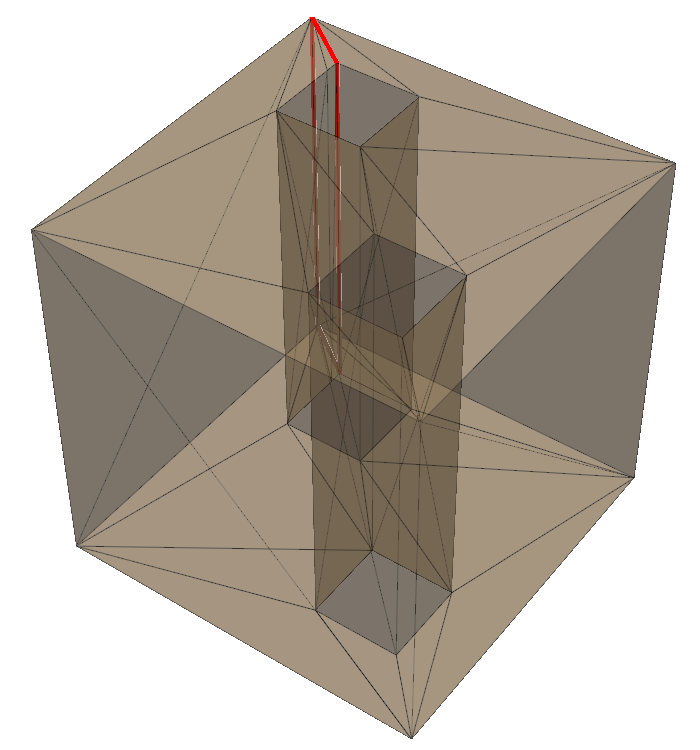
\includegraphics[width=\textwidth]{Genus2_2_optim_new.png}
        % \caption{提取经纬线后}
    \end{subfigure}
    \begin{subfigure}{.2\textwidth}
        \centering
        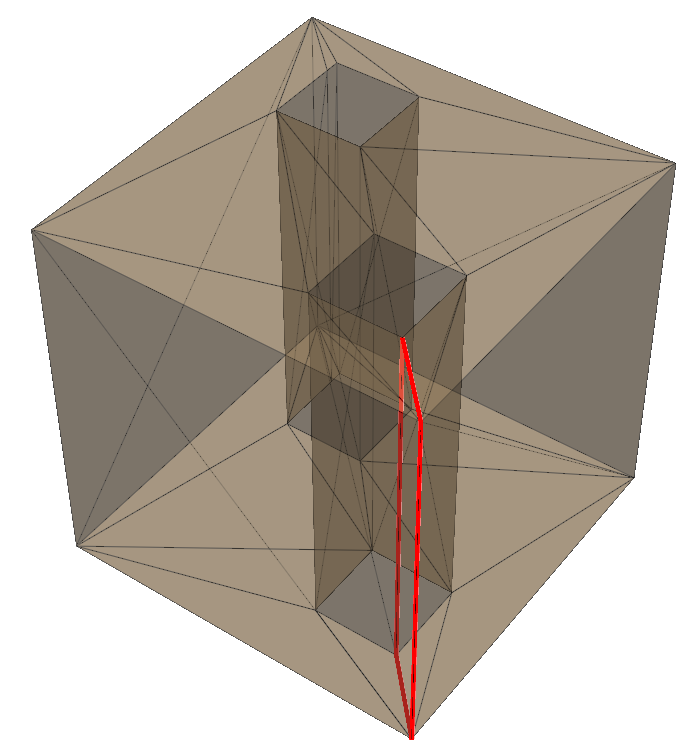
\includegraphics[width=\textwidth]{Genus2_3_optim_new.png}
        % \caption{提取经纬线后}
    \end{subfigure}
    \caption{Genus2 模型的最短同调圈,红色为同调基圈,共 4 个}
    \label{fig:genus2him}
\end{figure}

图 \ref{fig:eighthim} 展示了计算最短同调圈算法对 Eight 模型的输出。

\begin{figure}[h]
    \centering
    \begin{subfigure}{.2\textwidth}
        \centering
        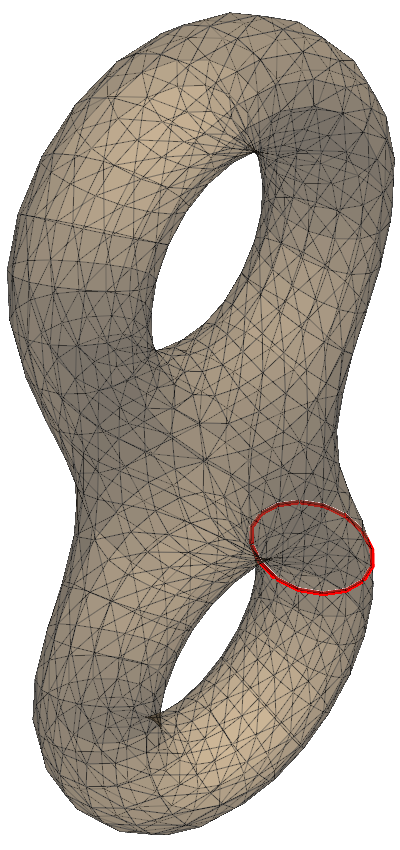
\includegraphics[width=\textwidth]{eight_0_optim_new.png}
        % \caption{提取经纬线前}
    \end{subfigure}
    \begin{subfigure}{.2\textwidth}
        \centering
        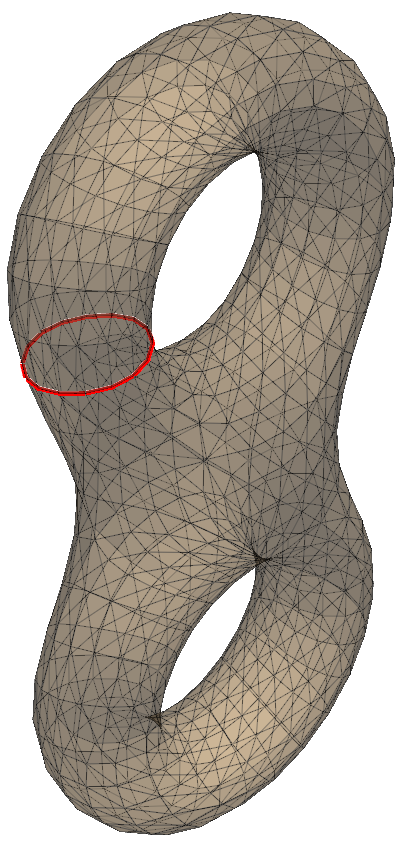
\includegraphics[width=\textwidth]{eight_1_optim_new.png}
        % \caption{提取经纬线后}
    \end{subfigure}
    \begin{subfigure}{.2\textwidth}
        \centering
        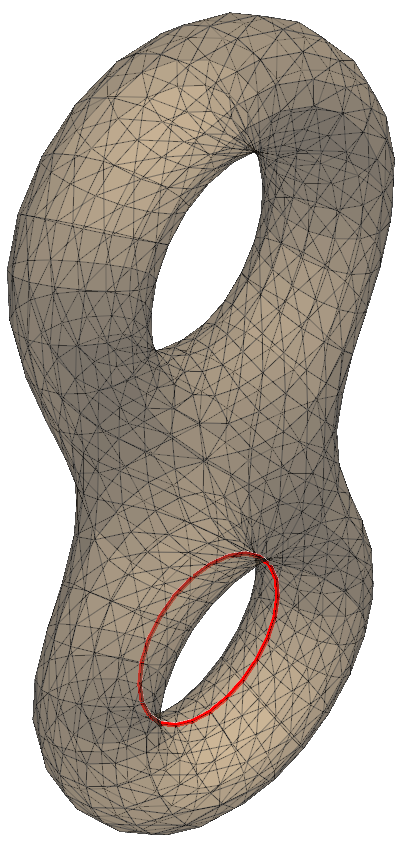
\includegraphics[width=\textwidth]{eight_2_optim_new.png}
        % \caption{提取经纬线后}
    \end{subfigure}
    \begin{subfigure}{.2\textwidth}
        \centering
        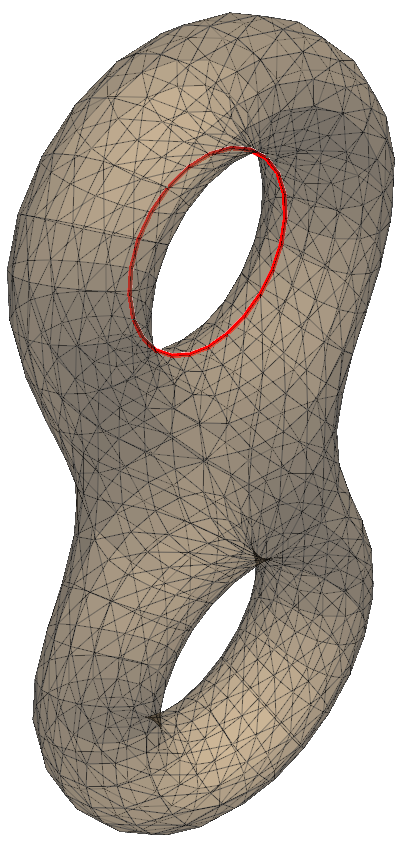
\includegraphics[width=\textwidth]{eight_3_optim_new.png}
        % \caption{提取经纬线后}
    \end{subfigure}
    \caption{Eight 模型的最短同调圈,红色为同调基圈,共 4 个}
    \label{fig:eighthim}
\end{figure}

可以看到,最短同调圈计算的实现在这两个例子下是正确的。

\begin{figure}[h]
    \begin{subfigure}{.5\textwidth}
        \centering
        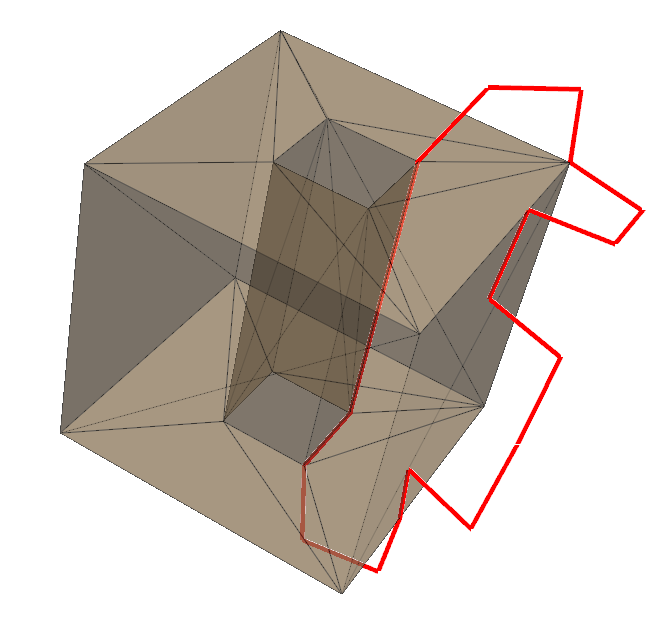
\includegraphics[width=\textwidth]{Genus1_han_basis.png}
        \caption{$ H_1(\mathbb{O}) $ 中的一个非零圈}
        \label{fig:hanh1o}
    \end{subfigure}
    \begin{subfigure}{.5\textwidth}
        \centering
        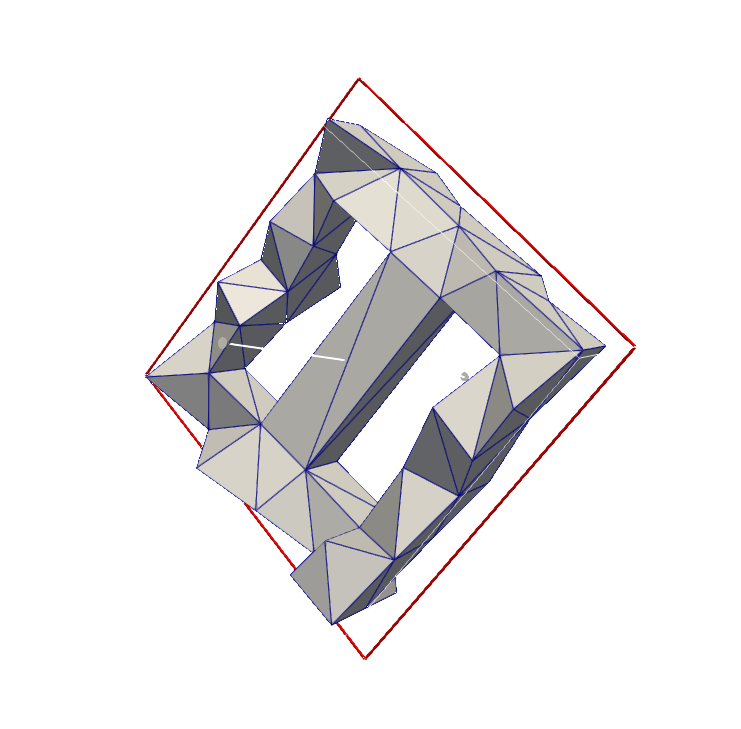
\includegraphics[width=\textwidth]{hanparaview.png}
        \caption{TetGen 后 $ \mathbb{O} $ 中的一个剖面}
        \label{fig:hanparaview}
    \end{subfigure}
    \caption{计算亏格为 1 模型的柄圈的部分步骤的结果}
\end{figure}

图 \ref{fig:hanh1o} 和图 \ref{fig:hanparaview} 展示了对亏格为 1 的模型计算柄圈的部分步骤的计算结果。图 \ref{fig:hanh1o} 中没有显示 $ \mathbb{O} $ 中除 $ \mathcal{M} $ 之外的四面体的面。

针对部分模型进行的最短同调圈计算性能测试见表 \ref{tab:perftable}。从表格中可以看到,最短同调圈的计算速度还不能满足较大模型的计算需求。

\begin{table}[h!]
    \centering
    \caption{部分模型的性能测试}
    \label{tab:perftable}
    \begin{tabular}{lllllll}
      \toprule
      模型名称 & V   & E    & F  & 亏格  & 候选圈数 & 最短同调圈计算用时 \\
      \midrule
      Genus1        & 16  & 48   & 32   & 1 & 528 & 0.187s \\
      Genus2        & 26  & 84   & 56   & 2 & 1534 & 0.464s \\
      Chair\_reduced & 488 & 1500 & 1000 & 7 & 494344 & 174.382s \\
      Eight         & 766 & 2304 & 1536 & 2 & 1178874 & 501.112s \\
      \bottomrule
    \end{tabular}
\end{table}

Genus1 进行三角剖分后的 (V, E, F) 分别为 (198, 1080, 2500)。当前版本的最短同调圈算法实现中,解 $ \mathbb{Z}_2 $ 下线性方程组是通过 numpy.linalg 中的 solve 方法在 $ \mathbb{R} $ 上计算,舍入到整数后再模 2 进行的。此方法受数值精度影响较大,在该剖分后 $ \mathcal{O} $ 的计算结果有误。

纯 Python 实现的 $ \mathbb{Z}_2 $ 域 Gauss 消元由于 Python 本身的开销,计算速度较浮点的 solve 方法慢 1 到 2 个数量级,而测试时间有限,所以没有得出柄圈计算的性能数据和最终结果。